
\documentclass[sigconf]{acmart}

\setcopyright{none}

\settopmatter{printacmref=false} % Removes citation information below abstract
\renewcommand\footnotetextcopyrightpermission[1]{} % removes footnote with conference information in first column
\pagestyle{plain} % removes running headers
  
\begin{document}
  
\title{\HUGE{\textbf{Traind AI Warfleet}}}

\author{Michel Schwarz}
\affiliation{\institution{Hochschule Düsseldorf}}
\email{michel.schwarz@study.hs-duesseldorf.de}

\author{Niklas Tluk}
\affiliation{\institution{Hochschule Düsseldorf}}
\email{niklas.tluk@study.hs-duesseldorf.de}

\begin{abstract}
 Summary of all aspects
\end{abstract}
  
\begin{CCSXML}
<ccs2012>
   <concept>
       <concept_id>10010147.10010257.10010258.10010261</concept_id>
       <concept_desc>Computing methodologies~Reinforcement learning</concept_desc>
       <concept_significance>100</concept_significance>
       </concept>
   <concept>
       <concept_id>10010147.10010257.10010282.10010291</concept_id>
       <concept_desc>Computing methodologies~Learning from critiques</concept_desc>
       <concept_significance>100</concept_significance>
       </concept>
   <concept>
       <concept_id>10010147.10010178.10010219.10010221</concept_id>
       <concept_desc>Computing methodologies~Intelligent agents</concept_desc>
       <concept_significance>100</concept_significance>
       </concept>
   <concept>
       <concept_id>10010147.10010257.10010293.10010294</concept_id>
       <concept_desc>Computing methodologies~Neural networks</concept_desc>
       <concept_significance>100</concept_significance>
       </concept>
 </ccs2012>
\end{CCSXML}

\ccsdesc[100]{Computing methodologies~Reinforcement learning}
\ccsdesc[100]{Computing methodologies~Learning from critiques}
\ccsdesc[100]{Computing methodologies~Intelligent agents}
\ccsdesc[100]{Computing methodologies~Neural networks}

%% Keywords. The author(s) should pick words that accurately describe
%% the work being presented. Separate the keywords with commas.
\keywords{intelligent systems, intelligent agents, deep reinforcment learning, neural networks}

%% A "teaser" image appears between the author and affiliation
%% information and the body of the document, and typically spans the
%% page.
\begin{teaserfigure}
 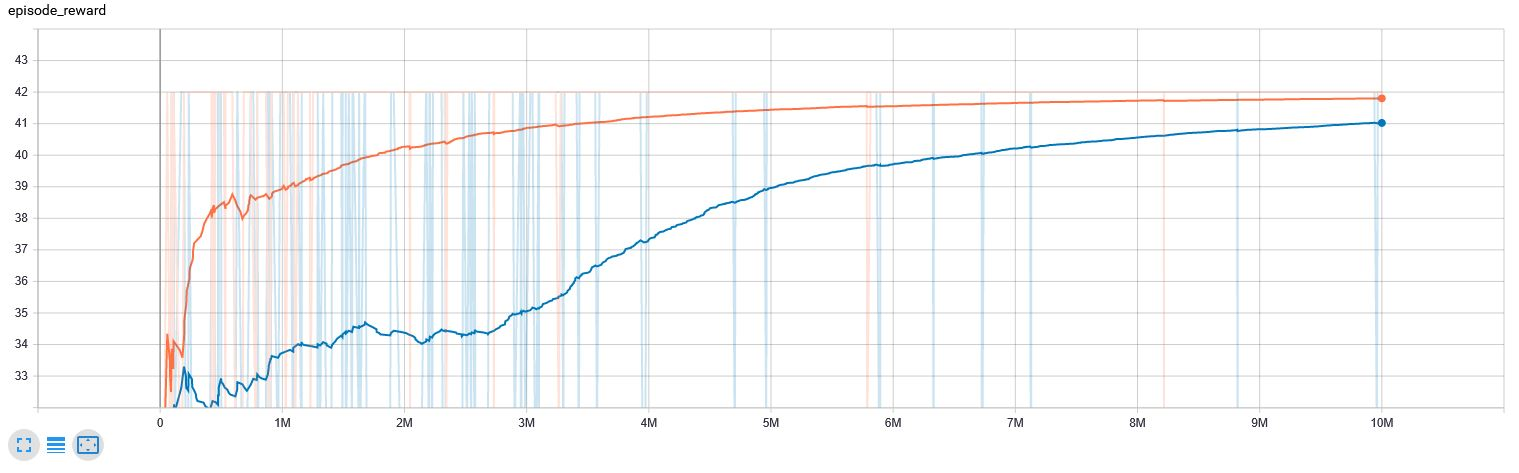
\includegraphics[width=\textwidth]{episode_reward_big}
  \caption{Episode Rewards A2C(Orange) and PPO2(Blue).}
  \Description{Enjoying the baseball game from the third-base
  seats. Ichiro Suzuki preparing to bat.}
  \label{fig:teaser}
\end{teaserfigure}

%%
%% This command processes the author and affiliation and title
%% information and builds the first part of the formatted document.
\maketitle 

\section{Introduction}
 This project is part of our participation in the intelligent systems course at the HSD in Düsseldorf, Germany.
 ...

\section{Motivation}
 ...

\section{Goal}
 Our goal is the implementation and training of an agent, capable of competently playing the board game warfleet, in python using reinforcement learning.
 ...

\section{Environment}
To achieve this we also had to develop a feasible environment for the agent to be trained in. For this purpose we chose the OpenAI Gym toolkit, which provides an easy-to-use suite of reinforcement learning tasks.
 ...

\section{Methods}
 agents, training, tests

\section{Implementation}
 ...
 
 \section{Results}
 ...
 
 \section{Conclusion}
  ...
  
  \section{Future Work}
Currently there are no plans for further development, with leaves the future of  this project as uncertain.


\end{document}